% !TeX root = linear-codes.tex
% !TEX TS-program = pdfLaTeX
\documentclass[10pt,letterpaper]{article}

\usepackage[utf8]{inputenc}
\usepackage{hyperref}
\usepackage{lmodern}
\usepackage{amsmath,amsthm,amssymb}
\usepackage{accents}
\usepackage{microtype}
\usepackage[hmargin=3.8cm,vmargin=2cm]{geometry}
\usepackage{xcolor}
\usepackage{nicefrac}
\usepackage{bbm}
\usepackage{aliascnt}
\usepackage{mathtools}
\usepackage{sectsty}
\usepackage{tikz}

\definecolor{Blue}{RGB}{5,55,77}
\definecolor{Red}{RGB}{20,50,10}
\definecolor{purple}{HTML}{8c3fcf}
\hypersetup{
    colorlinks,
    citecolor=Blue,
    filecolor=Blue,
    linkcolor=Blue,
    urlcolor=Blue,
    breaklinks=false,
}

\sectionfont{\large}
\subsectionfont{\normalsize}

\input{definitions/math}
\input{definitions/fields}
\input{definitions/probability}
\input{definitions/entropy}
\input{definitions/linearalgebra}
\input{definitions/theoremlike}
\input{definitions/citations}
\addbibresource{references/main.bib}

\newcommand{\vol}{\operatorname{Vol}}
\newcommand{\wt}{\operatorname{wt}}
\newcommand{\circuit}{\mathbb C}
\newcommand{\ball}{B_d}
\newcommand{\kero}{K}

\begin{document}
\title{\vspace{-35px}\bf\fontsize{15}{19}\selectfont
  Linear codes exceeding the Gilbert--Varshamov bound%
  \vspace{-5px}}
\author{\fontsize{10}{12}\selectfont
  Mert Saglam\\[-1pt]
  \fontsize{9}{11}\selectfont DeepInfra}
\date{}
\maketitle
\vspace{-18px}

% !TeX root = linear-codes.tex
\renewenvironment{abstract}{\small \list{}{%
    \setlength{\leftmargin}{10mm}%
    \setlength{\rightmargin}{\leftmargin}%
    \listparindent 0em%
  }\item\relax{\bf Abstract.}}{\endlist}

\begin{abstract}
Fix $\eps>0$, and let $n$, $d$ satisfy
$\lg n\ll d\le (1/2-\eps)n$. We show the existence of linear
codes over $\field_2^n$ of distance $d$ and size at least
$$
c_\eps n\,\frac{2^n}{\sum_{i=1}^{d-1}\binom ni}
$$
for some $c_\eps>0$ depending on $\eps$ only, which is
$\Omega(n)$ times the Gilbert--Varshamov bound. Our proof is
a straightforward refinement of the folklore union-bound
argument and gives the largest known linear codes in the
regime $e\sqrt{n}+\Omega(\lg n) \le d \le (1/2-\eps)n$.
\end{abstract}


% More
%precisely, our proof gives
%$$
%(1-o(1))\frac{\ln(2^n/V)}4\frac{2^n}{V}.
%$$
%In particular, when $d=o(n)$ the improvement factor is
%$(\ln 2/4-o(1))n$.
\vspace{13px}
\noindent\emph{In memory of Erik Palmgren (1963--2019)}
\vspace{-5px}
% !TeX root = linear-codes.tex
\section{Introduction}
\label{sec:intro}
In this paper we exhibit binary linear codes of blocklength
$n$ and size $\Omega(n)$ times the Gilbert--Varshamov
bound for any distance $d$ in the range
$\lg n\ll d\le(1/2-\eps)n$. Denote
\begin{align*}
  \ball=\setbuilder{x\in\field_2^n}{0<|x|<d}
\end{align*}
the set of all 0-1 vectors with weight between 1 and $d-1$,
and set $V=|\ball|$. The Gilbert--Varshamov bound
\cite{Gilbert1952, Varshamov1957} says that there exists a
code of size at least
\begin{align*}
  \frac{2^n}{V+1},
\end{align*}
and such a code may be chosen to be linear
\cite{Varshamov1957}. For fixed relative distance $d/n$,
Jiang and Vardy \cite{JiangV2004} obtained a superconstant
multiplicative improvement by exhibiting nonlinear codes
whose size is $\Omega(\lg V)$
times the Gilbert--Varshamov bound. The improvement is
$\Omega(n)$ when $d/n$ is a constant and $\Omega(d\lg(n/d))$
for $d\ll n$.

Gaborit and Zémor \cite{GaboritZ2008} obtained an
$\Omega(n)$ improvement for linear codes, but only at rate
$1/2$ and for certain blocklengths $n=2p^m$. The rate
parameter $1/2$ corresponds to distance
$d=\delta_0n+\Theta(\lg n)$, where $\delta_0\approx0.11$ is
the constant satisfying $\entb{\delta_0}=1/2$. More
recently, Hao, Huang, Livshyts, and Tikhomirov
\cite{HaoHLT2022} obtained an $\Omega(\sqrt n)$ improvement
for general binary linear codes at fixed relative distance
$d/n$. Yuan and Zhu \cite{YuanZ2026} gave another proof of
the same $\Omega(\sqrt n)$ improvement and extended the
result to quantum codes.
%
% !TeX root = linear-codes.tex
% The binary matrix-vector product illustrated with marks and empty cells.
\begin{center}
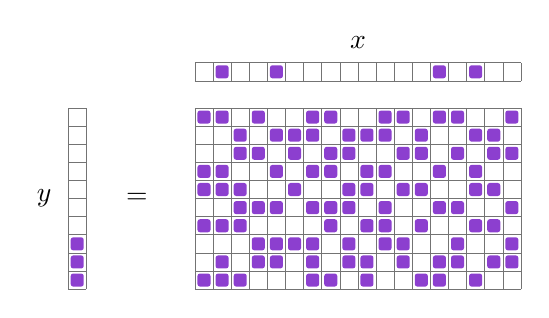
\begin{tikzpicture}[x=2.3mm,y=2.3mm]
  \tikzset{binary grid line/.style={
    draw=black!55,
    line width=.22pt,
    line cap=butt
  }}
  \def\zeromarkhalfwidth{.36}
  \def\zeromarkcorner{.90pt}

  % Draw a binary grid from row-major data, with the top row first.
  % Arguments: lower-left x, lower-left y, rows, columns, data.
  % Ones are centered purple rounded squares that do not touch the cell walls.
  % The complete grid is drawn afterward as
  % rows+1 uninterrupted horizontal lines and columns+1 vertical lines.
  \newcommand{\drawbinarygrid}[5]{%
    \path[fill=white] (#1,#2) rectangle ++(#4,#3);
    \edef\binarydata{#5}
    \foreach \bit [count=\cell from 0] in \binarydata {%
      \pgfmathtruncatemacro{\gridrow}{int(\cell/#4)}
      \pgfmathtruncatemacro{\gridcol}{mod(\cell,#4)}
      \ifnum\bit=1\relax
        \path[fill=purple,rounded corners=\zeromarkcorner]
          ({#1+\gridcol+.5-\zeromarkhalfwidth},
           {#2+#3-\gridrow-.5-\zeromarkhalfwidth})
          rectangle
          ({#1+\gridcol+.5+\zeromarkhalfwidth},
           {#2+#3-\gridrow-.5+\zeromarkhalfwidth});
      \fi
    }
    \foreach \gridrow in {0,...,#3} {
      \draw[binary grid line]
        (#1,{#2+\gridrow}) -- ++(#4,0);
    }
    \foreach \gridcol in {0,...,#4} {
      \draw[binary grid line]
        ({#1+\gridcol},#2) -- ++(0,#3);
    }
  }

  \def\matrixrows{10}
  \def\matrixcols{18}
  \def\matrixleft{7}
  \def\matrixbottom{1}

  \def\xdata{0,1,0,0,1,0,0,0,0,0,0,0,0,1,0,1,0,0}
  \def\ydata{0,0,0,0,0,0,0,1,1,1}
  \def\matrixdata{
    1,1,0,1,0,0,1,1,0,0,1,1,0,1,1,0,0,1,
    0,0,1,0,1,1,1,0,1,1,1,0,1,0,0,1,1,0,
    0,0,1,1,0,1,0,1,1,0,0,1,1,0,1,0,1,1,
    1,1,0,0,1,0,1,1,0,1,1,0,0,1,0,1,0,0,
    1,1,1,0,0,1,0,0,1,1,0,1,1,0,0,1,1,0,
    0,0,1,1,1,0,1,1,1,0,1,0,0,1,1,0,0,1,
    1,1,1,0,0,0,0,1,0,1,1,0,1,0,0,1,1,0,
    0,0,0,1,1,1,1,0,1,0,1,1,0,0,1,0,0,1,
    0,1,0,1,1,0,1,0,1,1,0,1,0,1,1,0,1,1,
    1,1,1,0,0,0,1,1,0,1,0,0,1,1,0,1,0,0
  }

  % Derive the layout from the matrix dimensions.
  \pgfmathsetmacro{\matrixcenterx}{\matrixleft+\matrixcols/2}
  \pgfmathsetmacro{\matrixcentery}{\matrixbottom+\matrixrows/2}
  \pgfmathsetmacro{\matrixtop}{\matrixbottom+\matrixrows}
  \pgfmathsetmacro{\xgridbottom}{\matrixtop+1.5}
  \pgfmathsetmacro{\xgridtop}{\xgridbottom+1}
  \pgfmathsetmacro{\legendheight}{\matrixbottom-.45}

  % x is aligned with the matrix columns and separated by 1.5 cells.
  \drawbinarygrid{\matrixleft}{\xgridbottom}
    {1}{\matrixcols}{\xdata}
  \drawbinarygrid{0}{\matrixbottom}
    {\matrixrows}{1}{\ydata}
  \drawbinarygrid{\matrixleft}{\matrixbottom}
    {\matrixrows}{\matrixcols}{\matrixdata}

  \node[left=2.5pt] at (0,\matrixcentery) {$y$};
  \node at (3.8,\matrixcentery) {$=$};
  \node[above=1.5pt] at (\matrixcenterx,\xgridtop) {$x$};
\end{tikzpicture}

\vspace{2mm}
{\footnotesize The filled cells of $x$ select columns of $M$;
their sum is $y=Mx$.}
\end{center}

%

We show that a straightforward refinement of the folklore
union-bound argument gives an $\Omega(n)$ multiplicative
improvement to the Gilbert--Varshamov bound uniformly
throughout the range $\lg n\ll d\le(1/2-\eps)n$. This
establishes the largest known linear codes for
$e \sqrt{n} + \Omega(\lg n)\le d \le (1/2-\eps)n$.
%
Recall that a linear code of size $2^{n-r}$ may be specified
through its parity check matrix $H\in\field_2^{r\times n}$
satisfying $Hx \ne 0$ for all $x\in \ball$. Let $M$ be
chosen uniformly at random from $\field_2^{r\times n}$ and
put $\kero=\setbuilder{x\in \ball}{Mx = 0}$. By linearity of
expectation,
%
$\E\sparen{\size{\kero}}=\size{\ball}2^{-r}$.
%
When $r>\lg\size{\ball}$, we get
$\Pr\sparen{\kero\neq\emptyset} \le \E\sparen{\size{\kero}}<
1$, therefore an $r\times n$ parity check matrix for a
distance $d$ code is guaranteed to exist, which is the
folklore union-bound argument.

If we choose $r = \lg\size{\ball}-\lg(cn)$ instead, we have
$\E[\size{\kero}]=cn$ and we can no longer use the union
bound to argue $\Pr[\kero=\emptyset]>0$. We show that, for
small enough $c$, there is a choice of $M$ for which $\kero$
contains no odd circuit, that is, no inclusion-minimal
linearly dependent subset of odd cardinality. This allows
us to extend $M$ with just one more carefully chosen
parity-check row which maps all elements of $\kero$ to
nonzero. Indeed, every dependency among the elements of
$\kero$ then has even cardinality. Thus, if $\mathbf K$ is
the matrix whose columns are the elements of $\kero$, the
all-ones row lies in its row space, and
$v\mathbf K=\mathbf{1}^\transpose$ has a solution.
Extending $M$ with such a row $v$ gives the desired matrix.
A slight modification also proves linear independence of
$\kero$, with slightly worse intermediate constants; see
Remark~\ref{rem:linear-independence}.

% !TeX root = linear-codes.tex
\section{Circuits and walks}
\label{sec:approach}

Put $w=d-1$.
Fix $\eps>0$.  We work in the range
$$
\ln n\ll w\le(1/2-\eps)n.
$$
Define the redundancy parameter
$$
R\defeq\ln\frac{2^n}{V}.
$$
Our assumptions imply $R=\Theta(n)$.  Fix
$0<\zeta<1$, and choose the integer $m$ so that, with
$$
\tau\defeq V2^{-m},
$$
we have
$$
\frac{(1-\zeta)R}{2}
\le\tau<(1-\zeta)R.
$$
Such an $m$ exists because this interval has multiplicative width
two.

Choose $M$ uniformly from $\field_2^{m\times n}$ and put
$$
\kero\defeq\setbuilder{x\in\ball}{Mx=0}.
$$
A \emph{circuit} in $\ball$ is an inclusion-minimal linearly
dependent subset.  If $\circuit_\ell$ is the collection of
$\ell$-element circuits in $\ball$, then every
$S\in\circuit_\ell$ satisfies
$$
\sum_{x\in S}x=0,
\qquad
\rank(S)=\ell-1,
$$
where $3\le\ell\le n+1$.

Define the probability kernel
$$
\mu(x)\defeq\frac{\indicate{x\in\ball}}{V}.
$$
Let $X_1,X_2,\ldots$ be independent with law $\mu$, and set
$$
p_\ell\defeq\Pr[X_1+\cdots+X_\ell=0].
$$
Every circuit in $\circuit_\ell$ gives $\ell!$ distinct ordered
tuples counted by this event.  Hence
$$
\size{\circuit_\ell}
\le\frac{V^\ell}{\ell!}p_\ell.
$$

Let $Z$ be the number of odd circuits contained in $\kero$.
Since the span of an $\ell$-element circuit has dimension
$\ell-1$,
$$
\Pr[S\subseteq\ker M]
=2^{-m(\ell-1)}
=\nparen{\frac{\tau}{V}}^{\ell-1}.
$$
Consequently,
$$
\begin{aligned}
\E Z
&=\sum_{\substack{3\le\ell\le n+1\\\ell\text{ odd}}}
  \size{\circuit_\ell}
  \left(\frac{\tau}{V}\right)^{\ell-1}\\
&\le\frac V\tau
  \sum_{\substack{\ell\ge3\\\ell\text{ odd}}}
  \frac{\tau^\ell}{\ell!}p_\ell.
\end{aligned}
$$

It suffices to find a choice of $M$ for which $Z=0$.  Indeed,
every zero-sum subset can be partitioned into circuits.  Hence, if
$\kero$ contains no odd circuit, then every dependency among its
elements has even cardinality.  Let $\mathbf K$ be the matrix whose
columns are the elements of $\kero$.  The preceding statement means
that
$$
\mathbf K a=0
\quad\Longrightarrow\quad
\mathbf1^\transpose a=0.
$$
Thus $\mathbf1^\transpose$ lies in the row space of $\mathbf K$,
and there is a row vector $v$ satisfying
$$
v\mathbf K=\mathbf1^\transpose.
$$
Appending $v$ to $M$ then produces a parity-check matrix for a
distance-$d$ code.

We now express the sum above as a transition probability.  Let
$J_t$ be Poisson with mean $t$, independently of the $X_i$, and
define the continuous-time random walk on $\field_2^{n+1}$ by
$$
W_t\defeq\sum_{i=1}^{J_t}(X_i,1).
$$
The walk starts at zero.  Write
$$
e_{n+1}\defeq(0,\ldots,0,1).
$$
Conditioning on the number of steps gives
$$
e^\tau\Pr[W_\tau=e_{n+1}]
=
\sum_{\substack{\ell\ge3\\\ell\text{ odd}}}
\frac{\tau^\ell}{\ell!}p_\ell,
$$
where the one-step term vanishes because $0\notin\ball$.
Consequently,
$$
\E Z
\le
\frac{Ve^\tau}{\tau}\Pr[W_\tau=e_{n+1}].
$$
It remains to prove
$$
\Pr[W_\tau=e_{n+1}]
<\frac{\tau e^{-\tau}}{V}.
$$

% !TeX root = linear-codes.tex
\section{The transition probability}

\subsection{Fourier analysis on the cube}
For functions $f,g \colon\field_2^n\to\reals$, let
$\iprod{f}{g}=\sum_x f(x)g(x)$. Define the Fourier basis
functions $\chi_y$ for $y\in\field_2^n$ as
$\chi_y(x) = (-1)^{x\cdot y}$. Note that
$\iprod{\chi_y}{\chi_y}=2^n$ and for $y\neq z$ we have
$\iprod{\chi_y}{\chi_z}=0$.
We define the Fourier transform of a function
as the coefficients in this character basis:
$$
\hat f(y) = \iprod{f}{\chi_y}.
$$
Note our Fourier transform is $2^{n/2}$ times a unitary.
The inverse transform is thus $2^{-n/2}$ times a unitary
given by
$$
f = \E_y\sparen{\hat f(y)\chi_y}.
$$

\subsection{Fourier estimates for Hamming balls}

The following two consequences of the sharp moment and tail
bounds of Kirshner and Samorodnitsky \cite[Corollary 1.4 and
Theorem 1.5]{KirshnerS2021} are all that we need.  Their
derivation is given in \autoref{sec:moment-tail-derivation}.

\begin{lemma}[Fourier estimates for the punctured Hamming
ball]
\label{lem:ball-fourier-estimates}
Let $w=d-1$, and let
$$
\mu(x)=\frac{\indicate{x\in\ball}}{V}.
$$
Fix $\eps>0$ and suppose
$$
\lg n\ll w\le(1/2-\eps)n.
$$
Then
$$
\E_y\abs{\hat\mu(y)}^3
=O\left(\frac1{Vn^3}\right)
$$
and
$$
\Pr_y\sparen{\abs{\hat\mu(y)}>1/n}
\le
2^{-n+\frac{2n\lg n}{w}
\lg\nparen{\frac{ew}{\lg n}}}.
$$
\end{lemma}

\subsection{Proof of the transition estimate}

Fourier inversion gives
$$
p_\ell=\E_y\hat\mu(y)^\ell.
$$
It follows from the identity in the preceding section that
$$
\Pr[W_\tau=e_{n+1}]
=e^{-\tau}\E_y\sinh\nparen{\tau\hat\mu(y)}.
$$
Moreover,
$$
\E_y\hat\mu(y)=\mu(0)=0.
$$
Set
$$
s(z)\defeq\sinh z-z.
$$
We therefore have
$$
\Pr[W_\tau=e_{n+1}]
=e^{-\tau}\E_y s\nparen{\tau\hat\mu(y)}.
$$

We shall use
$$
s(z)\le0\quad(z\le0),
\qquad
s(z)\le(\sinh1-1)z^3\quad(0\le z\le1),
\qquad
s(z)\le\frac12e^z\quad(z\ge1).
$$
Since $\abs{\hat\mu(y)}\le1$, it follows that
$$
\Pr[W_\tau=e_{n+1}]
\le
(\sinh1-1)e^{-\tau}\tau^3
\E_y\abs{\hat\mu(y)}^3
+
\frac12\Pr_y[\hat\mu(y)>1/\tau].
$$

Since
$$
\tau<R\le n\ln2<n,
$$
the first term is
$$
O\nparen{\frac{e^{-\tau}}V}.
$$
Since $\tau=\Theta(n)$, for all sufficiently large $n$ this is
less than
$$
\frac{\tau e^{-\tau}}{2V}.
$$

For the second term, put
$$
\theta\defeq
\frac{2\lg n}{w}\lg\nparen{\frac{ew}{\lg n}}.
$$
Our assumption $w\gg\lg n$ implies $\theta\longrightarrow0$.
The same lemma gives
$$
\Pr_y\sparen{\hat\mu(y)>1/\tau}
\le
\Pr_y\sparen{\abs{\hat\mu(y)}>1/n}
\le2^{-n(1-\theta)}.
$$
Since $R=\Theta(n)$, for all sufficiently large $n$ we have
$n\theta\ln2\le\zeta R/2$.  Therefore
$$
\begin{aligned}
\frac{\frac12 2^{-n(1-\theta)}}
     {\tau e^{-\tau}/V}
&=
\frac1{2\tau}
\exp\left(-R+\tau+n\theta\ln2\right)\\
&\le
\frac1{2\tau}e^{-\zeta R/2}
<\frac12
\end{aligned}
$$
for all sufficiently large $n$.  This proves
the desired transition bound, and hence $\E Z<1$.

Some choice of $M$ therefore has no odd circuit in $\kero$.
Appending the corresponding row $v$ described in the preceding
section produces a distance-$d$ code of size at least
$$
2^{n-m-1}
=\frac{\tau2^n}{2V}
\ge
\frac{(1-\zeta)R}{4}\frac{2^n}{V}.
$$
Thus, for every fixed $0<\zeta<1$ and all sufficiently large $n$,
there is a code $C$ satisfying
$$
\size{C}
\ge
\frac{1-\zeta}{4}
\ln\nparen{\frac{2^n}{V}}\frac{2^n}{V}.
$$
As $\zeta$ can be chosen arbitrarily small, there are codes for
which
$$
\liminf_{n\longrightarrow\infty}
\frac{4V\size{C}}{2^n\ln(2^n/V)}\ge1.
$$
For example, if $d/n\longrightarrow1/5$, then the multiplicative
improvement over the Gilbert--Varshamov bound satisfies
$$
\liminf_{n\longrightarrow\infty}
\frac1n\frac{\size{C}}{2^n/V}
\ge
\frac{\ln2}{4}\nparen{1-\entb{1/5}}
=0.048\ldots.
$$

\begin{remark}
\label{rem:linear-independence}
A slight modification also shows that $\kero$ is linearly
independent, with slightly larger numerical constants in the
estimates but no loss in the leading asymptotic constant.
Let $Z_{\mathrm{all}}$ count all circuits in $\kero$, and put
$\phi(z)=e^z-1-z-z^2/2$. The circuit count and Fourier
inversion give
$$
\E Z_{\mathrm{all}}
\le\frac V\tau\sum_{\ell\ge3}\frac{\tau^\ell}{\ell!}p_\ell
=\frac V\tau\E_y\phi\nparen{\tau\hat\mu(y)}.
$$
We have $\phi(z)\le0$ for $z\le0$,
$\phi(z)\le(e-5/2)z^3$ for $0\le z\le1$, and
$\phi(z)\le e^z$ for $z\ge1$. Splitting at
$\hat\mu(y)=1/\tau$ and applying
\autoref{lem:ball-fourier-estimates} as above yields
$$
\begin{aligned}
\E Z_{\mathrm{all}}
&\le(e-5/2)V\tau^2\E_y\abs{\hat\mu(y)}^3
  +\frac{Ve^\tau}{\tau}\Pr_y[\hat\mu(y)>1/\tau]\\
&\le O(1/\tau)+\frac{e^{-\zeta R/2}}{\tau}
=o(1).
\end{aligned}
$$
Thus $\kero$ is linearly independent with probability $1-o(1)$
for the same choice of $m$.
\end{remark}

\printbibliography
\appendix
% !TeX root = linear-codes.tex
\section{Derivation of the moment and tail estimates}
\label{sec:moment-tail-derivation}

We derive \autoref{lem:ball-fourier-estimates} from
\cite[Corollary 1.4 and Theorem 1.5]{KirshnerS2021}.
Put $\rho=w/n$.  The third-moment specialization of their moment bound
says that every polynomial $f$ of degree at most $w$ satisfies
$$
\E|f|^3
\le
(\E f^2)^{3/2}
2^{n(\entb{\rho}/2-\gamma(\rho))},
$$
where
$$
\begin{aligned}
\gamma(\rho)\defeq{}&
-\frac{\rho}{2}\lg \rho-2(1-\rho)\lg(1-\rho)-1\\
&+\left(1-\frac{3\rho}{2}\right)\lg(2-3\rho).
\end{aligned}
$$
Indeed, the auxiliary parameter in their moment exponent satisfies
$$
1-2u=\sqrt{\frac{\rho}{2-3\rho}},
$$
and substitution gives the displayed expression.  Elementary
calculus gives
$$
\gamma'(\rho)
=\frac12\lg\frac{(1-\rho)^4}{\rho(2-3\rho)^3}.
$$
It follows that $\gamma$ is strictly positive on $(0,1/2)$ and
$$
\gamma(\rho)=\frac{\rho}{2}\lg\frac1\rho+O(\rho)
\qquad(\rho\longrightarrow0).
$$
Consequently, for every fixed $\eta>0$, there is a constant
$c_\eta>0$ such that
$$
\gamma(\rho)\ge c_\eta \rho\lg\frac1\rho
\qquad
\left(0<\rho\le\frac12-\eta\right).
$$
As a function of the signs
$((-1)^{x_1},\ldots,(-1)^{x_n})$, the function
$\widehat\mu(x)$ is a multilinear polynomial of degree at most
$w$.  Moreover, Parseval's identity and Stirling's formula give
$$
\E_x\widehat\mu(x)^2=\frac1V,
\qquad
\lg V=n\entb{\rho}+O(\lg n).
$$
Applying the preceding moment estimate to $\widehat\mu$ gives
$$
\begin{aligned}
Vn^2\E_x|\widehat\mu(x)|^3
&\le
n^2V^{-1/2}
2^{n\entb{\rho}/2-c_\eta w\lg(n/w)}\\
&=
2^{-c_\eta w\lg(n/w)+O(\lg n)}
=O(1/n),
\end{aligned}
$$
where the last equality follows from $w\gg\ln n$.
This proves the moment estimate in
\autoref{lem:ball-fourier-estimates}.

We next derive the tail estimate.  For
$$
0\le y\le\frac12-\sqrt{\rho(1-\rho)}
$$
define
$$
T(\rho,y)
\defeq
\entb{\rho}+
\int_0^y
\lg\left(
\frac{1-2\rho+\sqrt{(1-2\rho)^2-4z(1-z)}}{2(1-z)}
\right)\,dz.
$$
Kirshner and Samorodnitsky's tail bound says that, when $ny$ is an
integer,
$$
\Pr\left[
|f|\ge
\sqrt{\E f^2}\,
2^{n(T(\rho,y)-\entb{\rho}/2)}
\right]
\le
2^{n(\entb{y}-1)}.
$$
The expression inside the logarithm defining $T$ is at most
$1-2\rho$.  Therefore
$$
\entb{\rho}-T(\rho,y)
\ge y\lg\frac1{1-2\rho}
\ge\frac{2\rho y}{\ln2}.
$$

Take
$$
y=\frac1n\left\lceil\frac{n\lg n}{w}\right\rceil.
$$
Our assumption $w\gg\ln n$ gives $y\longrightarrow0$, so the
permitted range for $y$ holds for all sufficiently large $n$.
The standard estimate
$$
V\ge\binom nw\ge\frac{2^{n\entb{\rho}}}{n+1}
$$
and the preceding bound on $T$ give
$$
\begin{aligned}
V^{-1/2}2^{n(T(\rho,y)-\entb{\rho}/2)}
&\le
\sqrt{n+1}\,2^{n(T(\rho,y)-\entb{\rho})}\\
&\le
\sqrt{n+1}\,2^{-2wy/\ln2}\\
&\le
\sqrt{n+1}\,n^{-2/\ln2}\\
&\le\frac1n
\end{aligned}
$$
for all sufficiently large $n$.  Hence the threshold in the
tail bound is at most $1/n$.  Moreover,
$$
y\le\frac{\lg n}{w}+\frac1n
\le\frac{2\lg n}{w}.
$$
Using $\entb{y}\le y\lg(e/y)$, we conclude that
$$
\begin{aligned}
\Pr_x\sparen{|\widehat\mu(x)|>1/n}
&\le
2^{-n+n\entb{y}}\\
&\le
2^{-n+\frac{2n\lg n}{w}
\lg\left(\frac{ew}{\lg n}\right)}.
\end{aligned}
$$
This proves the tail estimate and completes the derivation of
\autoref{lem:ball-fourier-estimates}.

\section*{AI methodology statement}
The main proof was discovered by the author. ChatGPT-6.1 Sol
assisted with editing the manuscript and the matrix-vector
illustration in the introduction, checking mathematical
arguments and references, and drafting the linear-independence
argument in Remark~\ref{rem:linear-independence}. The author
takes full responsibility for the correctness and originality
of the paper, including all AI-assisted content and references.
\end{document}
